\documentclass[a4paper, 12pt]{article}
\usepackage[utf8]{inputenc}
\usepackage[T1]{fontenc}
\usepackage{lmodern}
\usepackage[slovene]{babel}
\usepackage{amsmath, amssymb, amsthm}
\usepackage{graphicx}
\usepackage{hyperref}
\usepackage{enumitem}
\usepackage{float}
\usepackage{caption}
\usepackage{geometry}


\def\N{\mathbb{N}} % mnozica naravnih stevil
\def\Z{\mathbb{Z}} % mnozica celih stevil
\def\Q{\mathbb{Q}} % mnozica racionalnih stevil
\def\R{\mathbb{R}} % mnozica realnih stevil
\def\C{\mathbb{C}} % mnozica kompleksnih stevil

\newtheorem{definicija}{Definicija}
\newtheorem{izrek}[definicija]{Izrek}
\newtheorem{trditev}[definicija]{Trditev}
\newtheorem{posledica}[definicija]{Posledica}
\newtheorem{lema}[definicija]{Lema}
\newtheorem{opomba}[definicija]{Opomba}
\newtheorem{zgled}[definicija]{Zgled}


\title{Permutacijsko-pošteni\\ nabori kock}
\author{Lan Stare\\
Fakulteta za matematiko in fiziko \\
Oddelek za matematiko}
\date{11.\ maj 2025}

\begin{document}

\maketitle

\section{Uvod}

Kocke so že stoletja vir zabave, iger na srečo in matematičnega zanimanja. Na prvi pogled je poštenost kocke preprost pojem: če vržemo kocko z $n$ ploskev, naj bo vsaka izmed njih enako verjetna. Takšna definicija zadostuje pri klasičnih igrah, kjer nas zanima verjetnost določenega izida.

A kaj se zgodi, če poštenost razumemo v kontekstu primerjav med kockami? Predstavljajmo si igro, kjer vsak igralec vrže svojo kocko in zmaga tisti, ki dobi višje število.

\begin{definicija}
  Nabor kock $K = \{K_1, K_2, \ldots, K_n\}$ ima \textbf{poštenost prvega}, če ima vsaka izmed kock (oziroma igralec) enako verjetnost za zmago.
\end{definicija}

\begin{definicija}
  Nabor kock $K = \{K_1, K_2, \ldots, K_n\}$ ima \textbf{poštenost mesta}, če imajo vse kocke enako verjetnost, da bodo zasedle katerokoli mesto v vrstnem redu izidov.
\end{definicija}

Poštenosti mesta seveda implicira poštenost prvega, saj če so vse kocke enako verjetne, potem je tudi verjetnost, da bo katerakoli kocka zmagala, enaka.

% Ali bi bilo mogoče, da neka kocka $A$ pogosteje premaga kocko $B$, $B$ pogosteje premaga kocko $C$, a $C$ pogosteje premaga kocko $A$? Ta nenavadna situacija ni le teoretična\,--\,gre za znani primer \emph{neprehodnih kock}, ki presenetljivo nasprotujejo intuiciji.

Po drugi strani si lahko predstavljamo situacijo, kjer želimo, da igra med več igralci ne daje prednosti nobenemu igralcu, ne glede na to, kako si razdelijo vloge ali vrstni red. V tem kontekstu nastopi zanimiv pojem {\em permutacijske poštenosti}.

\begin{definicija}
  Nabor kock $K = \{K_1, K_2, \ldots, K_n\}$ je \textbf{permutacijsko-pošten}, če ima vsaka permutacija kock glede na izide metov enako verjetnost.
\end{definicija}

Permutacijsko-poštenost je moč razumeti kot splošitev poštenosti mesta, kjer ne gledamo le na posamezne izide, temveč na celoten sistem metov kock. To pomeni, da ne glede na to, kako so kocke razporejene ali katero permutacijo izberemo, bo verjetnost vrstnega reda izidov vedno enaka. Poštenost mesta pomeni, da ko trije igralci: Bor, Ema in Lovro, vržejo kocke, imajo vsi enako verjetnost, da bodo 1., 2. ali pa 3. Permutacijska poštenost pa pove, da ima vrstni red igralcev Bor -> Ema -> Lovro enako verjetnost kot recimo Ema -> Bor -> Lovro. Permutacijska poštenost torej implicira poštenost mesta (in posledično tudi poštenost prvega).

\section{Permutacijsko-pošteni nabori kock}
Obstaja več načinov, kako lahko definiramo permutacijsko-poštene nabori kock. Če se samo osredotočimo na običajne 6-strane kocke, hitro vidimo, da za več kot 2 igralca nabor ni permutacijsko-pošten. To je namreč zato, ker če dva igralca po prvem metu vržeta enako število, potem morata za zmago metati ponovno, vendar potem tretji igralec ne more zmagati, saj je njegova kocka že iz igre. Zato se moramo najprej znebiti ponovitvam števil na kockah. Tudi na 6-stranih kockah ne moramo ostati, saj že za recimo 5 igralcev nabor 6-stranih kock ne more biti permutacijsko-pošten.

\begin{trditev}
  Za 5 igralcev ne obstaja permutacijsko-pošten nabor 6-stranih kock.
\end{trditev}

{\em Dokaz:\/}
  Predpostavimo, da obstaja permutacijsko-pošten nabor $K = \{K_1, K_2, K_3, K_4, K_5\}$, kjer so vse kocke 6-strane. Na vseh stranicah morajo biti različna števila, drugače bi lahko prišlo do enakih izidov, kar bi pomenilo, da nabor ne bi bil permutacijsko pošten. Če 5 igralcev meče 6-strane kocke, je torej $6^5$ možnih izidov. Teh $6^5$ različnih izidov pa mora biti deljivo s številom igralcev, če hočemo, da ima vsaka kocka enako strani. Število $6^5 = 2^5 * 3^5$ pa ni deljivo s 5.
\qed\\


Iskanje permutacijsko-poštenega nabora kock lahko posplošimo na iskanje nehomogenega nabora, kjer lahko igralec naenkrat meče več kock z različnim številom strani. Več o takih kockah si bomo pogledali na koncu v zaključku. Mi se bomo posvetili permutacijsko-poštenim naborom, ki imajo enako število ploskev (kot smo videli, bo to s številom igralcev naraščalo). Prav posebaj bomo poskušali odgovoriti na naslednji vprašanji:
\begin{itemize}
  \item Ali obstajajo permutacijsko-pošteni nabori kock z enakim številom stranic za poljubno število igralcev?
  \item Kako jih sistematično konstruirati?
\end{itemize}

\section{Obstoj permutacijsko-poštenih naborov}

Za začetek si poglejmo primer permutacijsko-poštenega nabora kock za 3 igralce. Vzemimo tri kocke $A$, $B$ in $C$, ki imajo naslednje ploskev:
\begin{itemize}
  \item Kocka $A$: 1, 6, 8, 12, 13, 17
  \item Kocka $B$: 2, 4, 9, 11, 15, 16
  \item Kocka $C$: 3, 5, 7, 10, 14, 18
\end{itemize}
%DODAJ SLIKO

Vsaka kocka ima 6 ploskev, na katerih so sama različna števila. Za ta nabor lahko preverimo, da je permutacijsko pošten.

\begin{opomba}
  Število kock bomo označevali z $n$, število ploskev na kockah pa z $d$. V našem primeru imamo $n = 3$ in $d = 6$. Takemo naboru kock bomo rekli 3d6.
\end{opomba}

Za poljuben $n$ bomo kazali, da obstaja permutacijsko-pošten nabor kock z $d$ ploskvami na vsaki kocki. Za to bomo uporabili konstrukcijo, ki temelji na permutacijah in kombinatoriki.

\begin{trditev}
  Za $n = 3$ obstaja permutacijsko-pošten nabor kock z $d \in \mathbb{N}$ ploskvami na vsaki kocki.
\end{trditev}

{\em Dokaz:\/}
  Za Tudi za $n = 3$ lahko uporabimo zgornje kocke:
  \begin{itemize}
  \item Kocka $A$: 1, 6, 8, 12, 13, 17
  \item Kocka $B$: 2, 4, 9, 11, 15, 16
  \item Kocka $C$: 3, 5, 7, 10, 14, 18
\end{itemize}

Ta nabor je že permutacijsko-pošten, a smo ga našli z golo silo, zato si poglejmo, ali lahko splošno konstruiramo nabor kock za 3 igralce.

Najlažje si bomo konstrukcijo predstavljali, če zapišemo kocke v niz. Torej razvrstimo števila v vrsto in namesto vrednosti zapišemo ime osebe/kocke, ki ima to vrednost na svoji kocki. Za naš primer dobimo: ABCBCACABCBAACBBAC.

Niz je permutacijsko pošten, če je število vsake trojice enako. Torej če preštejemo vse pojavitve ABC, ACB, BAC, BCA, CAB IN CBA v tem nizu in je število njih enako, potem je naš nabor permutacijsko pošten.

Lahko opazimo, da lahko naš niz razdelimo na trojice, ki so ravno vse različne permutacije niza ABC.
%RECI CHATU DA TI NARISE SLIKICO TEGA OZIROMA JO VZEMI IZ PP

Poskusimo zamenjati vrstni red teh trojic in jih ponovno zlepiti. Če ponovno preštejemo število vsake trojice, bomo ugotovili, da nov niz na žalost ni permutacijsko pošten. Torej tako ne moremo konstruirati poljubnega permutacijsko poštenega nabora, lahko pa v novem nizu opazimo nekaj drugega. Preštejmo število vsakega para: AB, AC, BA, BC, CA, CB v novem nizu. Izkaže se, da je vseh parov enako. Razlog za to je, da so vse trojice le permutirane verzije osnovnega niza ABC. Ko recimo preštevamo število ponovitev AB, lahko iz vsake trojice vzamemo največ eno črko, torej najprej vzamemo A iz prve in B iz druge trojice, nato A iz prve in B iz tretje trojice in tako naprej. Vseh teh možnosti pojavitev AB je $5 + 4 + 3 + 2 + 1$. Druga možnost, kje se AB lahko pojavita, je v isti trojici. Teh je 3. Očitno je, da za vsak par s tem postopkom dobimo 18 pojavitev. Ugotovili smo torej, da je število parov v tem nizu enako.

Zdaj pa zapišimo ta niz še 6-krat ($3!$). Na vsakem nizu dolžine 18 zdaj opravimo drugo permutacijo črk in vse nize poljubno zlepimo v en niz dolžine $6 * 18$. Če preštejemo zdaj število vseh trojic, bomo videli, da jih je enako.

Razmisliko, zakaj to drži. Število pojavitev niza ABC lahko podobno kot prej preštejemo glede na to, iz kje prihajajo črke A, B in C:
\begin{enumerate}
  \item lahko pridejo iz vsakega niza dolžine 18 posebaj 
  \item lahko sta AB skupaj in C v svojem nizu
  \item lahko sta BC skupaj in A v svojem nizu
  \item lahko je cel niz ABC v istem nizu
\end{enumerate}

Za niz BAC velja enako. V 1. se število ABC in BAC ujemata, ker je število vseh črk v nizih dolžine 18 enako. V 2. in 3. se ujemata zaradi prejšnjega argumenta, ko smo pokazali, da se ravno v teh nizih dolžine 18 število vseh parov ujema. Cel niz pa se pojavi enakokrat vse skupaj, saj so nizi dolžine 18 samo permutirana različica osnovnega niza z dolžino 18, v katerem smo permutirali črke.

\begin{izrek}
  Za vsak $n \geq 3$ obstaja permutacijsko-pošten nabor kock z $d \in \mathbb{N}$ ploskvami na vsaki kocki.
\end{izrek}

{\em Dokaz:\/}
Za $n = 3$ smo že pokazali, da obstaja permutacijsko-pošten nabor kock z $d = 6$ ploskvami na vsaki kocki. Za $n = 4$ lahko uporabimo enak postopek, le da bomo začeli z osnovnim nizom ABCD. Ta postopek bomo posplošini lahko na poljubno število igralcev $n$ in dobimo permutacijsko-pošten nabor kock z $d \in \mathbb{N}$ ploskvami na vsaki kocki.

Začnemo z nizom dolžine $n$, kot smo pri treh igralcih vzeli ABC. Ta niz permutiramo na vse možne načine in dobimo $n!$ različnih nizov dolžine $n$. Te nize poljubno zlepimo skupej, da dobimo en niz dolžine $(n*(n!))$. V tem nizu je število \underline{parov} enako. Ko ta niz zapišemo še $n!$-krat, permutiramo črke in nize spet zlepimo skupaj, da dobimo niz dolžine $n*(n!)^2$, v katerem je število \underline{trojic} enako. Ta proces spet ponovimo in dobimo niz dolžine $n*(n!)^(n-1)$, ki je permutacijsko pošten. Ploskev v tem nizu je $(n!)^(n-1)$.

S to konstrukcijo smo torej posplošili trditev za 3 igralce na poljubno število igralcev $n \geq 3$.
\qed

\section{Izboljšana konstrukcija}

Čeprav smo s prejšnjo konstrukcijo dobili permutacijsko-pošten nabor kock, je ta nabor precej velik. Število ploskev na kockah je namreč $d = (n!)^{(n-1)}$, kar hitro postane zelo veliko. Na primer, za 4 igralce dobimo $d = 24^3 = 13824$ ploskev na vsaki kocki, za 5 igralcev pa že $d = 120^4 = 207360000$. To je seveda preveliko, da bi bilo praktično uporabno.
V tem delu bomo predstavili izboljšano konstrukcijo, ki omogoča manjše število ploskev na kockah, hkrati pa ohranja permutacijsko-poštenost.

Michael Purcell je v [\ref{purcell}], je metodo, ki smo jo ravnokar obravnavali, izboljšal. Dokazal je, da je na primer za 5 igralcev dovolj 120 strana kocka.

Za njegovo, tako imenovano {\em Združitveno konstrukcijo}, bomo najprej vpeljali m/n permutacijsko-poštenost.

\begin{definicija} Naj bo $K = \{K_1, K_2, \ldots, K_n\}$ nabor kock. Pravimo, da je $K$ \textbf{m/n permutacijsko-pošten}, če je vsaka podmnožica $m$ kock iz $K$ permutacijsko-poštena.
\end{definicija}

To pomeni, da če je nabor 4/6 permutacijsko-pošten, je nabor 6 kock 4/4 permutacijsko-pošten, 3/3 permutacijsko-pošten in tudi 2/2 permutacijsko-pošten, ni pa nujno 5/5 in 6/6 permutacijsko-pošten. To pa pomeni, da če vzamemo katerekoli 4 kocke iz nabor 6 kock, ki je 4/6 permutacijsko-pošten, bodo permutacijsko poštene. Prav tako velja za 3 in 2 kocki, ne pa nujno za 5 in 6 kock.

Konstrukcija, ki smo jo opisali v Trditvi 6, je pravzaprav iz 1/3 permutacijsko-poštenega nabora kock sestavili 2/3 permutacijsko-pošten nabor in na koncu še 3/3 permutacijsko-pošten nabor kock. Na začetku smo vzeli nabor ABC, ki predstavlja 3 1-strane kocke. Nato smo z njimi sestavili 2/3 permutacijsko-pošten nabor kock, ki je bil sestavljen iz 6 2-stranih kock. Na koncu smo te 2-strane kocke zlepili skupaj in dobili 3/3 permutacijsko-pošten nabor kock, ki je bil sestavljen iz 6 3-stranih kock.

Purcellova {\em Združitvena konstrukcija} sloni na tem, da če zlepimo skupaj \underline{točno določene} nabore $m/n$ permutacijsko-poštenih kock, lahko konstruiramo manjši nabor $(m+1)/n$ permutacijsko-poštenih kocke, kot smo ga v Izreku 7.




  

\section{Zanimivosti in odprta vprašanja}

Najprej nam v glavo stopita dve vprašanji:
\begin{itemize}
  \item Ali obstaja boljša metoda za konstrukcijo permutacijsko-poštenih naborov kock?
  \item Koliko je najmanjše število ploskev na kocki za dano naravno števino $n$, da je nabor še vedno permutacijsko-pošten?
\end{itemize}

Če pa raziskovanje permutacijsko-poštenih naborov kock razširimo še na nehomogene kocke, se nam odprejo še dodatna vprašanja, saj lahko uporabimo večje število kock z različnim številom ploskev. Na primer, če imamo 3 igralce, lahko uporabimo 6-strane, 8-strane in 10-strane kocke. Predstavljamo si lahko, da je iskanje takih naborov še bolj zapleteno, saj lahko kombiniramo različno število ploskev in različno strane kocke. Vendar pa je tudi tu mogoče najti permutacijsko-poštene nabore, čeprav so konstrukcije bolj zapletene.

\begin{zgled}
  Za 5 igralcev lahko na primer uporabimo naslednje kocke, ki so prikazane na sliki levo, kjer vsakemu igralcu pripadajo kocke iste barve.
  \begin{figure}[h]
    \centering
    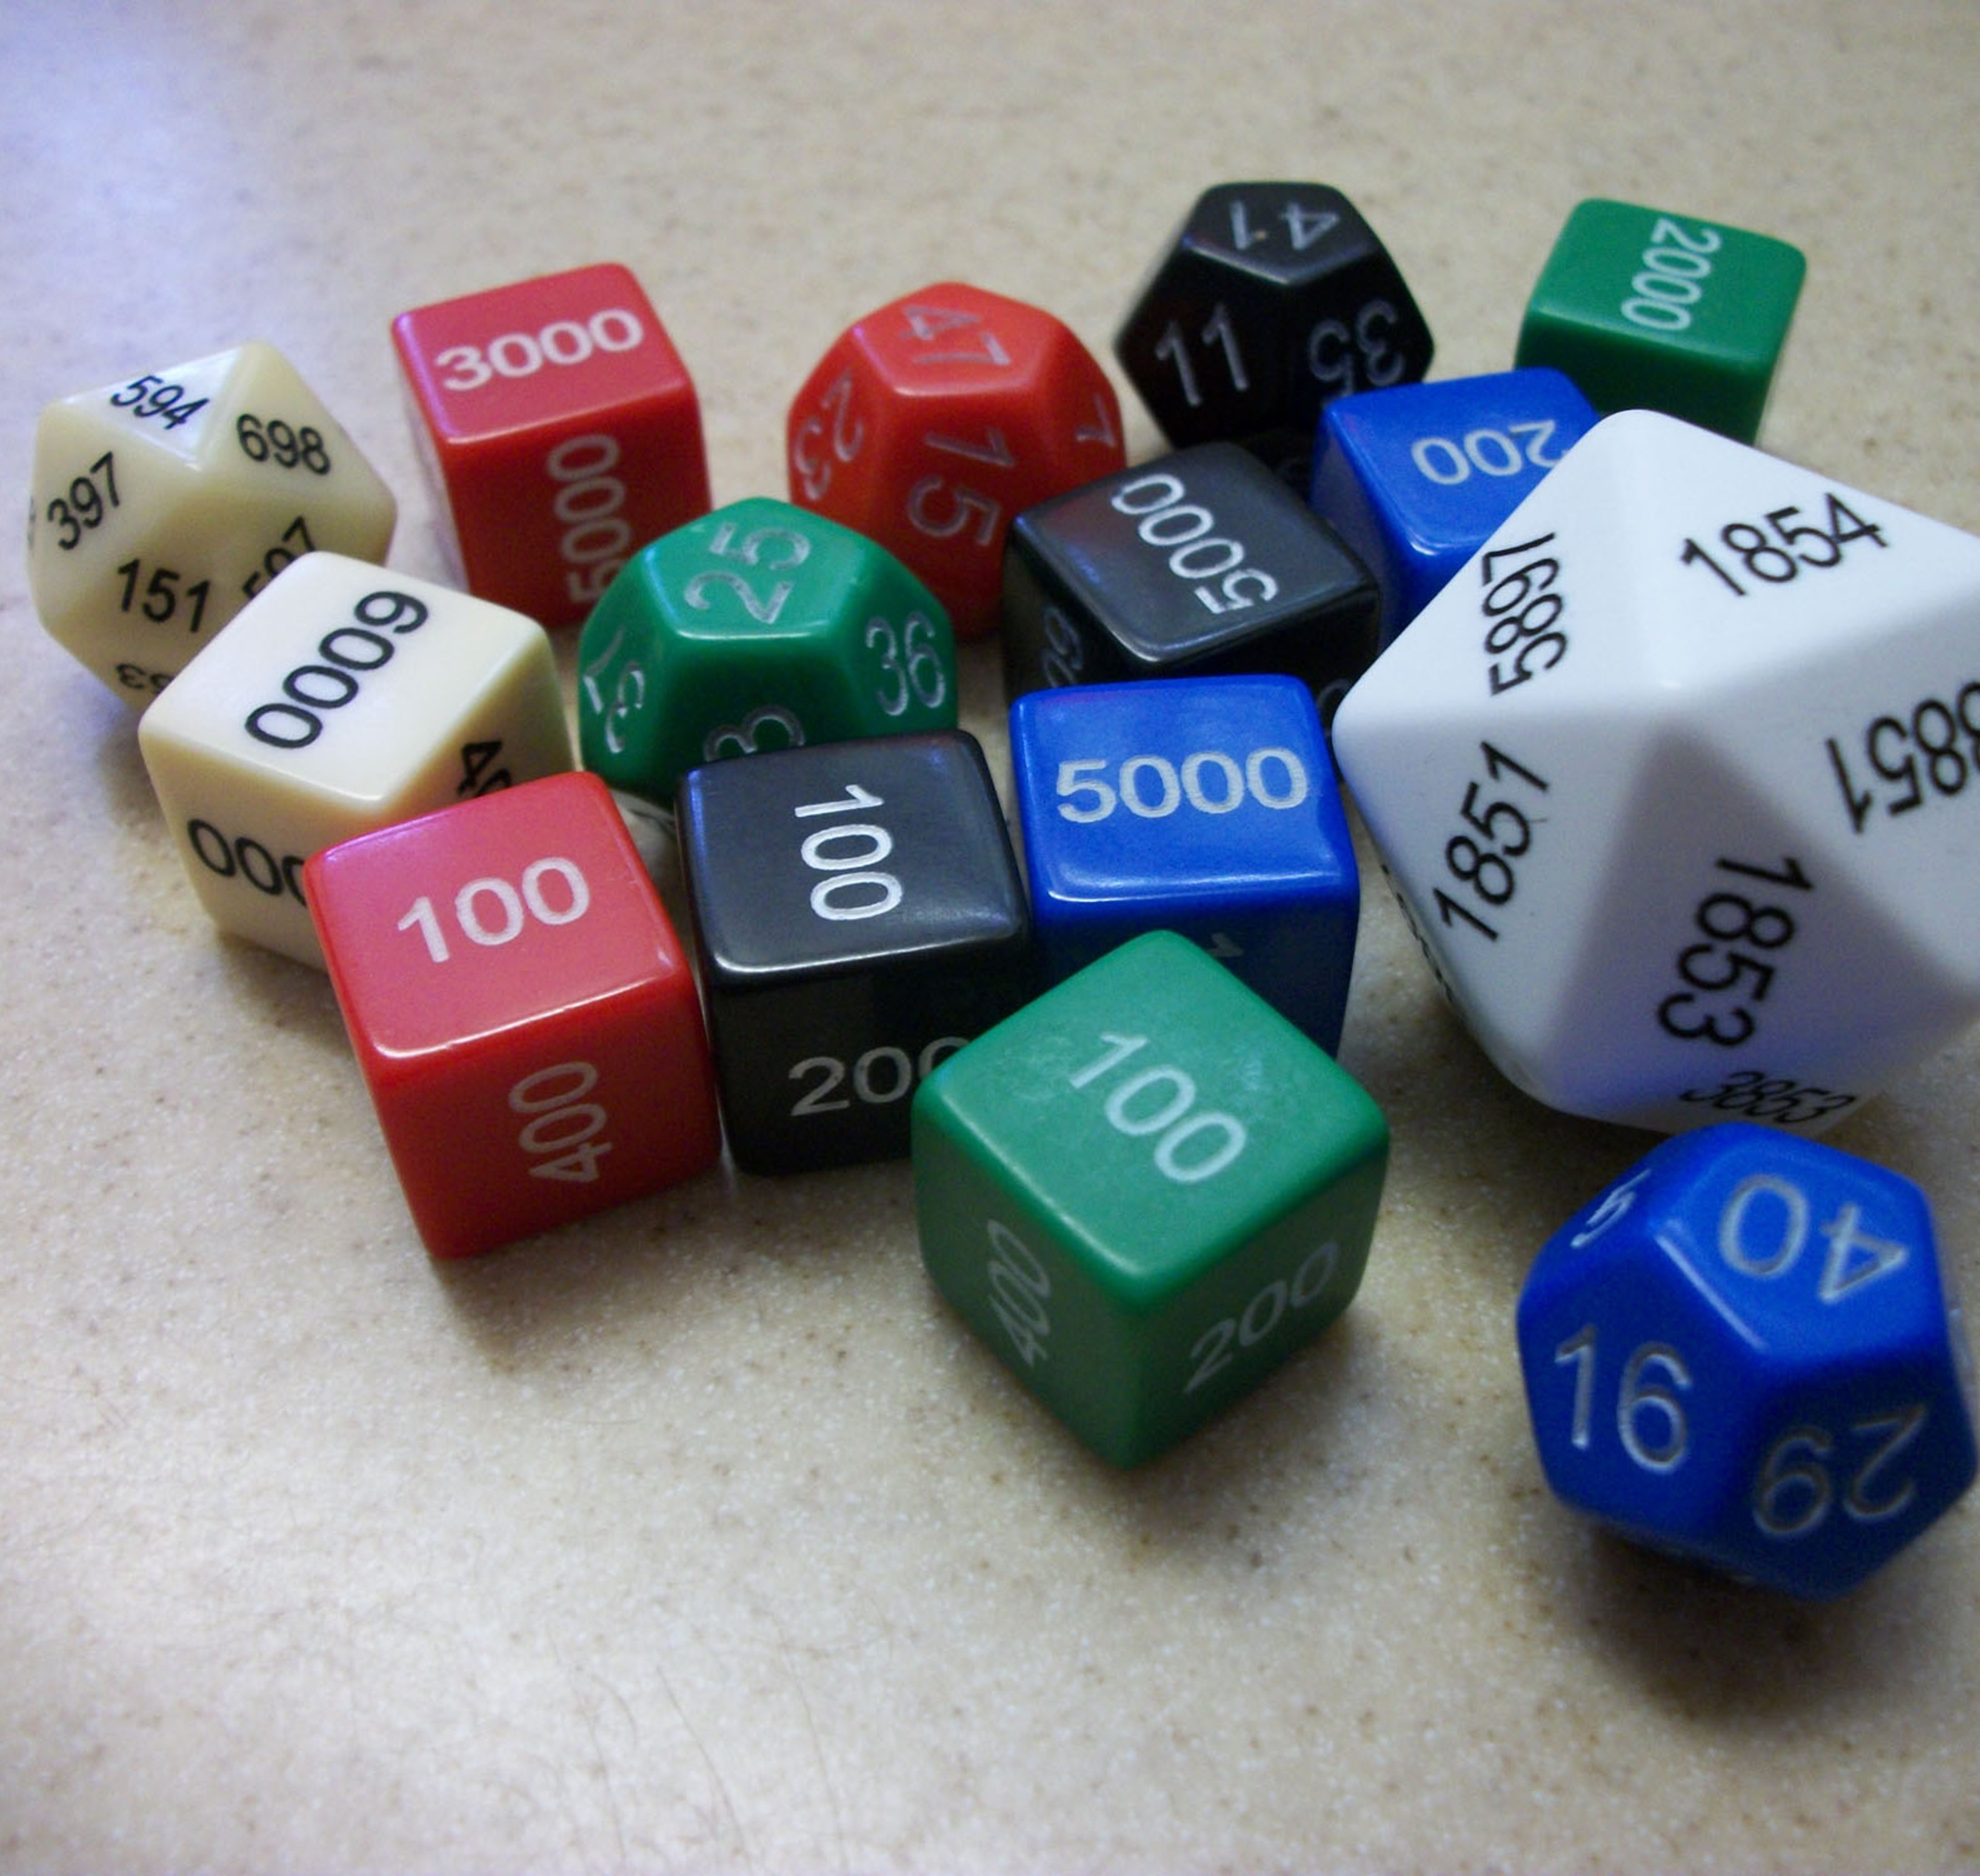
\includegraphics[width=0.45\textwidth]{Slike za pp/nehomogene_kocke.jpg}
    \caption{Nehomogen permutacijsko-pošten nabor kock za 5 igralcev.}
    \label{fig:nehomo_kocke}
  \end{figure}
\end{zgled}

\begin{zgled}
  Za poljubno število igralcev bi vedno lahko uporabili kocko, ki je prikazana v \ref{fig:ena_kocka}, ki ima $n!$ ploskev. Tako kocko mečemo natanko enkrat in permutacijsko-pošteno določi vrstni red igralcev.
  \begin{figure}[h]
    \centering
    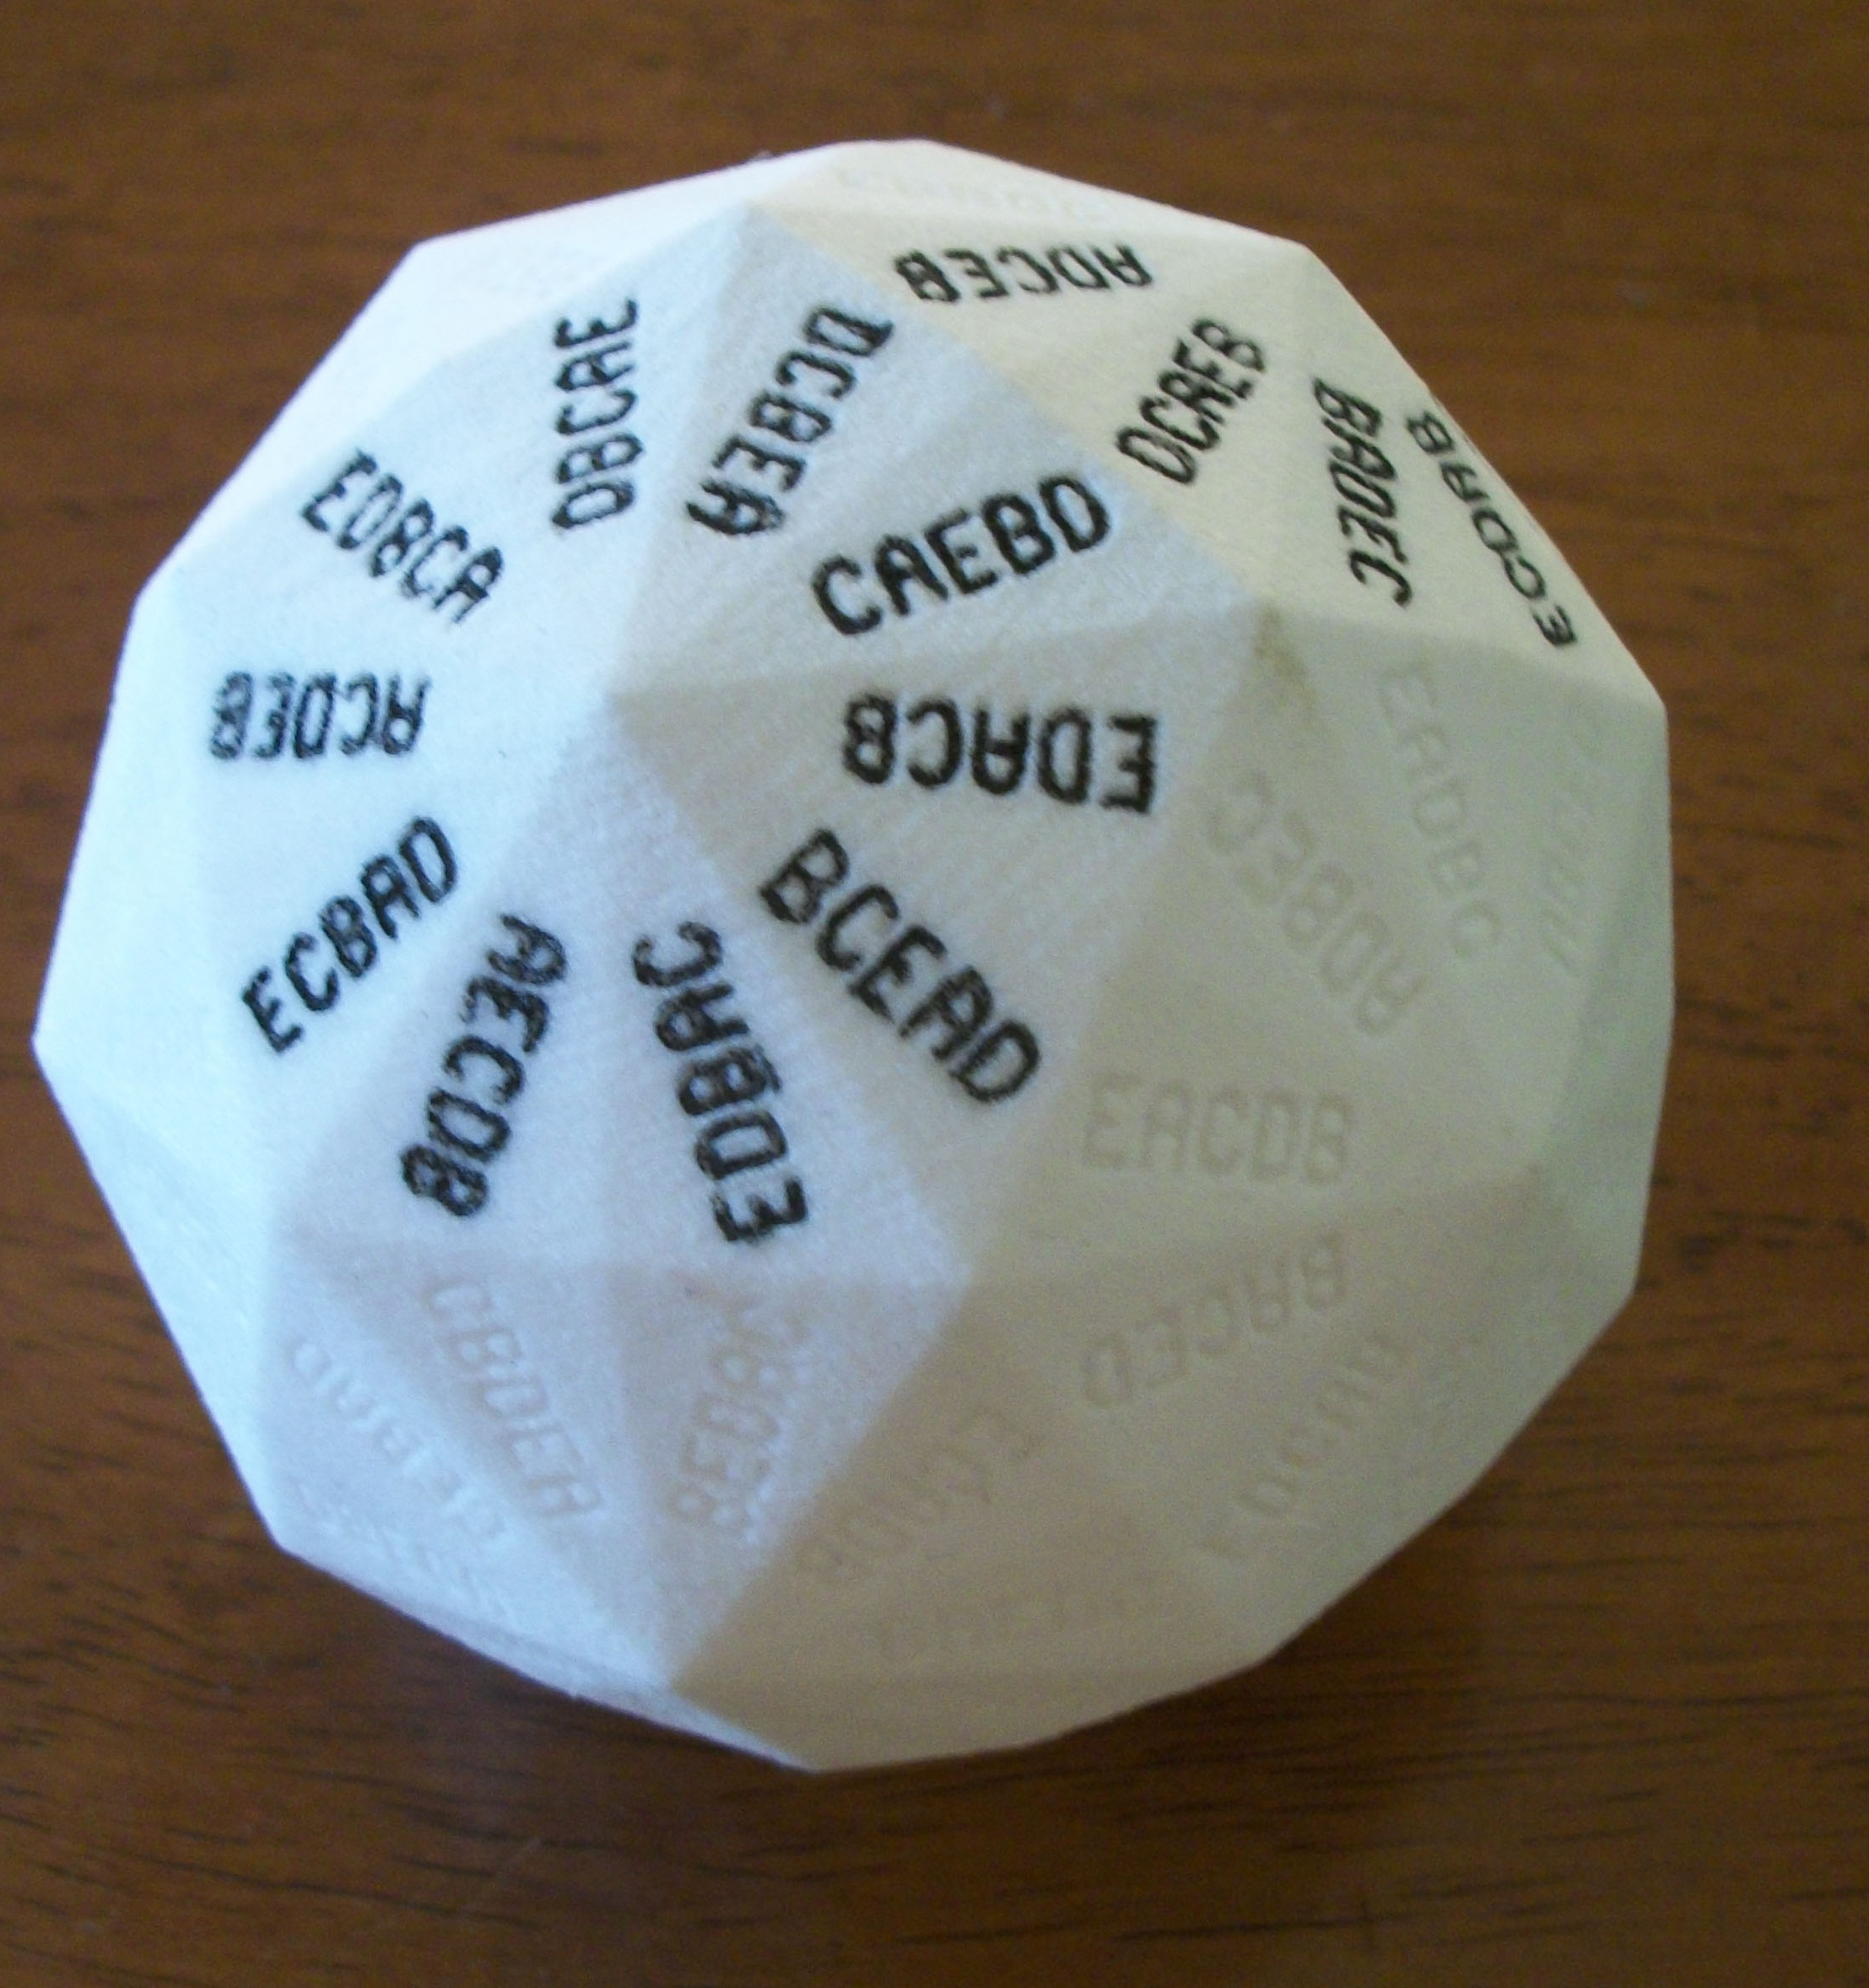
\includegraphics[width=0.45\textwidth]{Slike za pp/ena_kocka.jpg}
    \caption{Nehomogen permutacijsko-pošten nabor kock za 5 igralcev.}
    \label{fig:ena_kocka}
  \end{figure}
\end{zgled}

\section{Sklep}
Tema permutacijsko-poštenih naborov kock je zelo odprta in polna še neodgovorjenih vprašanj. Bogata je s kombinatornimi in verjetnostnimi izzivi, ki ponujajo širok spekter raziskovalnih možnosti. Permutacijsko-pošteni nabori kock so zanimivi ne le zaradi svoje teoretične vrednosti, temveč tudi zaradi praktične uporabnosti v igrah in simulacijah.

\section*{Literatura}
\begin{enumerate}
  \item \label{purcell} Michael Purcell, Building Sets of Permutation-Fair Dice, \emph{The American Mathematical Monthly}, 2024. \url{https://doi.org/10.1080/00029890.2024.2345576}
  \item Eric Harshbarger, \emph{Go first dice}, 2023. \url{http://www.ericharshbarger.org/dice/go_first_dice.html}
  \item Polylog, \emph{We designed special dice using math, but there's a catch}, 2022. \url{https://www.youtube.com/watch?v=-64UT8yikng&t=66s}
  \item SHU Recreational Maths Research Cluster, \emph{James Grime 'Go First Dice for five players and beyond' (SHU-RMRC Seminar 29th June 2020)}, 2021. \url{https://www.youtube.com/watch?v=L3d0YIW7wHU&t=1s}
  \item 
\end{enumerate}

\end{document}
